\section{Игрушечный декомпилятор}
\label{toy_decompiler}

\subsection{Введение}

Современный компилятор это результат работы сотен разработчиков/лет.
В то же время, игрушечный компилятор может быть упражнением для студента на неделю (или даже на выходные).

Точно также, коммерческий декомпилятор как Hex-Rays может быть невероятно сложным,
но игрушечный декомпилятор, как этот, может быть легко понят и сделан заново.

Нижеследующий декомпилятор написан на Питоне, поддерживает только короткие бейсик-блоки, без переходов.
Память также не поддерживается.

\subsection{Структура данных}

Наш игрушечный декомпилятор будет использовать только одну единственную структуру данных, которая представляет дерево выражений.

Многие учебники по программированию имеют пример конвертирования температуры из шкалы Фаренгейта в шкалу Цельсия, используя
такую формулу:

\begin{center}
{\large $celsius = (fahrenheit - 32) \cdot \frac{5}{9}$}
\end{center}

Это выражение может быть представлено как дерево:

% reworked from http://www.texample.net/tikz/examples/decision-tree/
\tikzset{
  treenode/.style = {shape=rectangle, rounded corners,
                     draw, align=center,
                     top color=white, bottom color=blue!20},
  env/.style      = {treenode, font=\ttfamily\normalsize},
}

\begin{center}
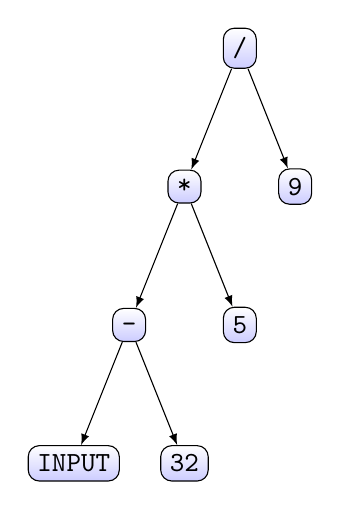
\begin{tikzpicture}
[
	grow                    = down,
	sibling distance        = 4em,
	level distance          = 5em,
	edge from parent/.style = {draw, -latex},
	every node/.style       = {font=\footnotesize},
	sloped
]
\node [env] {/}
	child
	{
		node [env] {*}
		child { 
			node [env] {-}
			child { node [env] {INPUT} }
			child { node [env] {32} }
			}
		child { node [env] {5} }
	}
	child { node [env] {9} }
	;

\end{tikzpicture}
\end{center}


Как хранить его в памяти?
Мы видим здесь 3 типа узлов: 1) числа (или значения); 2) арифметические операции; 3) символы (как ``INPUT'').

Многие разработчики, любящие использовать \ac{OOP}, создадут что-то вроде класса.
Другие разработчики, может быть, будут использовать ``variant type''.

Я буду использовать простейший способ представления этой структуры: Питоновский кортеж (tuple).
Первый элемент кортежа будет строкой:
``EXPR\_OP'' для операции, ``EXPR\_SYMBOL'' для символа, или ``EXPR\_VALUE'' для значения.
В случае с символом или значением, оно следует за строкой.
В случае операции, за строкой следуют другие кортежи.

Тип узла и тип операции хранятся как простые строки --- для облегчения отладки.

Вот \textit{конструкторы} в нашем коде, в \ac{OOP}-шном смысле.

\begin{lstlisting}
def create_val_expr (val):
    return ("EXPR_VALUE", val)

def create_symbol_expr (val):
    return ("EXPR_SYMBOL", val)

def create_binary_expr (op, op1, op2):
    return ("EXPR_OP", op, op1, op2)
\end{lstlisting}

Это также \textit{аксессоры}:

\begin{lstlisting}
def get_expr_type(e):
    return e[0]

def get_symbol (e):
    assert get_expr_type(e)=="EXPR_SYMBOL"
    return e[1]

def get_val (e):
    assert get_expr_type(e)=="EXPR_VALUE"
    return e[1]

def is_expr_op(e):
    return get_expr_type(e)=="EXPR_OP"

def get_op (e):
    assert is_expr_op(e)
    return e[1]

def get_op1 (e):
    assert is_expr_op(e)
    return e[2]

def get_op2 (e):
    assert is_expr_op(e)
    return e[3]
\end{lstlisting}

Выражение конвертирования температуры, которое мы только что видели, будет представлено как:

\begin{center}
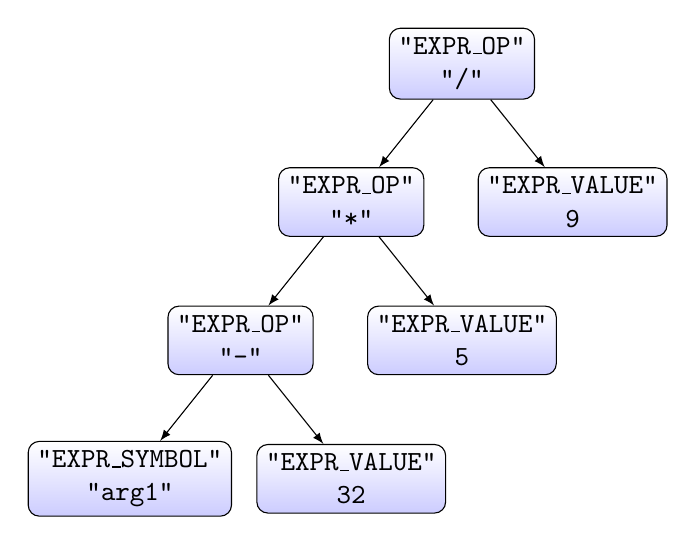
\begin{tikzpicture}
[
	grow                    = down,
	sibling distance        = 8em,
	level distance          = 5em,
	edge from parent/.style = {draw, -latex},
	every node/.style       = {font=\footnotesize},
	sloped
]
\node [env] {"EXPR\_OP"\\"/"}
	child
	{
		node [env] {"EXPR\_OP"\\"*"}
		child { 
			node [env] {"EXPR\_OP"\\"-"}
			child { node [env] {"EXPR\_SYMBOL"\\"arg1"} }
			child { node [env] {"EXPR\_VALUE"\\32} }
			}
		child { node [env] {"EXPR\_VALUE"\\5} }
	}
	child { node [env] {"EXPR\_VALUE"\\9} }
	;

\end{tikzpicture}
\end{center}


\dots или как Питоновское выражение:

\begin{lstlisting}
('EXPR_OP', '/', 
	('EXPR_OP', '*',
	('EXPR_OP', '-', ('EXPR_SYMBOL', 'arg1'), ('EXPR_VALUE', 32)), 
	('EXPR_VALUE', 5)), 
('EXPR_VALUE', 9))
\end{lstlisting}

На самом деле, это \ac{AST} в его простейшем виде.
\ac{AST} активно используются в компиляторах.

\subsection{Простые примеры}

Начнем с простейшего примера:

\begin{lstlisting}
        mov     rax, rdi
        imul    rax, rsi
\end{lstlisting}

В самом начале, такие символы присваиваются регистрами:
RAX=initial\_RAX,
RBX=initial\_RBX,
RDI=arg1,
RSI=arg2,
RDX=arg3,
RCX=arg4.

Когда мы обрабатываем инструкцию MOV, мы просто компируем выражение из RDI в RAX.
Когда мы обрабатываем инструкцию IMUL, мы просто создаем новое выражение, соеденяя вместе выражения из RAX и RSI
и сохраняя результат снова в RAX.

Я могу подать это на вход декомпилятору, и мы увидим, как состояние регистров меняется во время обработки:

\begin{lstlisting}
python td.py --show-registers --python-expr tests/mul.s

...

line=[mov       rax, rdi]
rcx=('EXPR_SYMBOL', 'arg4')
rsi=('EXPR_SYMBOL', 'arg2')
rbx=('EXPR_SYMBOL', 'initial_RBX')
rdx=('EXPR_SYMBOL', 'arg3')
rdi=('EXPR_SYMBOL', 'arg1')
rax=('EXPR_SYMBOL', 'arg1')

line=[imul      rax, rsi]
rcx=('EXPR_SYMBOL', 'arg4')
rsi=('EXPR_SYMBOL', 'arg2')
rbx=('EXPR_SYMBOL', 'initial_RBX')
rdx=('EXPR_SYMBOL', 'arg3')
rdi=('EXPR_SYMBOL', 'arg1')
rax=('EXPR_OP', '*', ('EXPR_SYMBOL', 'arg1'), ('EXPR_SYMBOL', 'arg2'))

...

result=('EXPR_OP', '*', ('EXPR_SYMBOL', 'arg1'), ('EXPR_SYMBOL', 'arg2'))
\end{lstlisting}

Инструкция IMUL связана со строкой ``*'', и затем новое выражение конструируется в
\TT{handle\_binary\_op()}, которая сохраняет результат в RAX.

В этом выводе, структуры данных выводятся используя Питоновскую ф-цию \TT{str()},
которая делает то же самое, что и \TT{print()}.

Вывод громоздкий, и мы можем выключить вывод Питоновских выражений и увидеть, как внутренняя структура данных аккуратно
выводится используя нашу внутреннюю ф-цию \TT{expr\_to\_string()}:

\begin{lstlisting}
python td.py --show-registers tests/mul.s

...

line=[mov       rax, rdi]
rcx=arg4
rsi=arg2
rbx=initial_RBX
rdx=arg3
rdi=arg1
rax=arg1

line=[imul      rax, rsi]
rcx=arg4
rsi=arg2
rbx=initial_RBX
rdx=arg3
rdi=arg1
rax=(arg1 * arg2)

...

result=(arg1 * arg2)
\end{lstlisting}

Более продвинутый пример:

\begin{lstlisting}
        imul    rdi, rsi
        lea     rax, [rdi+rdx]
\end{lstlisting}

Инструкция LEA обрабатывается просто как ADD.

\begin{lstlisting}
python td.py --show-registers --python-expr tests/mul_add.s

...

line=[imul      rdi, rsi]
rcx=('EXPR_SYMBOL', 'arg4')
rsi=('EXPR_SYMBOL', 'arg2')
rbx=('EXPR_SYMBOL', 'initial_RBX')
rdx=('EXPR_SYMBOL', 'arg3')
rdi=('EXPR_OP', '*', ('EXPR_SYMBOL', 'arg1'), ('EXPR_SYMBOL', 'arg2'))
rax=('EXPR_SYMBOL', 'initial_RAX')

line=[lea       rax, [rdi+rdx]]
rcx=('EXPR_SYMBOL', 'arg4')
rsi=('EXPR_SYMBOL', 'arg2')
rbx=('EXPR_SYMBOL', 'initial_RBX')
rdx=('EXPR_SYMBOL', 'arg3')
rdi=('EXPR_OP', '*', ('EXPR_SYMBOL', 'arg1'), ('EXPR_SYMBOL', 'arg2'))
rax=('EXPR_OP', '+', ('EXPR_OP', '*', ('EXPR_SYMBOL', 'arg1'), ('EXPR_SYMBOL', 'arg2')), ('EXPR_SYMBOL', 'arg3'))

...

result=('EXPR_OP', '+', ('EXPR_OP', '*', ('EXPR_SYMBOL', 'arg1'), ('EXPR_SYMBOL', 'arg2')), ('EXPR_SYMBOL', 'arg3'))
\end{lstlisting}

И снова, посмотрим, как это выражение может быть выведено более аккуратно:

\begin{lstlisting}
python td.py --show-registers tests/mul_add.s

...

result=((arg1 * arg2) + arg3)
\end{lstlisting}

Еще один пример, где используются 2 входных аргумента:

\begin{lstlisting}
        imul    rdi, rdi, 1234
        imul    rsi, rsi, 5678
        lea     rax, [rdi+rsi]
\end{lstlisting}

\begin{lstlisting}
python td.py --show-registers --python-expr tests/mul_add3.s

...

line=[imul      rdi, rdi, 1234]
rcx=('EXPR_SYMBOL', 'arg4')
rsi=('EXPR_SYMBOL', 'arg2')
rbx=('EXPR_SYMBOL', 'initial_RBX')
rdx=('EXPR_SYMBOL', 'arg3')
rdi=('EXPR_OP', '*', ('EXPR_SYMBOL', 'arg1'), ('EXPR_VALUE', 1234))
rax=('EXPR_SYMBOL', 'initial_RAX')

line=[imul      rsi, rsi, 5678]
rcx=('EXPR_SYMBOL', 'arg4')
rsi=('EXPR_OP', '*', ('EXPR_SYMBOL', 'arg2'), ('EXPR_VALUE', 5678))
rbx=('EXPR_SYMBOL', 'initial_RBX')
rdx=('EXPR_SYMBOL', 'arg3')
rdi=('EXPR_OP', '*', ('EXPR_SYMBOL', 'arg1'), ('EXPR_VALUE', 1234))
rax=('EXPR_SYMBOL', 'initial_RAX')

line=[lea       rax, [rdi+rsi]]
rcx=('EXPR_SYMBOL', 'arg4')
rsi=('EXPR_OP', '*', ('EXPR_SYMBOL', 'arg2'), ('EXPR_VALUE', 5678))
rbx=('EXPR_SYMBOL', 'initial_RBX')
rdx=('EXPR_SYMBOL', 'arg3')
rdi=('EXPR_OP', '*', ('EXPR_SYMBOL', 'arg1'), ('EXPR_VALUE', 1234))
rax=('EXPR_OP', '+', ('EXPR_OP', '*', ('EXPR_SYMBOL', 'arg1'), ('EXPR_VALUE', 1234)), ('EXPR_OP', '*', ('EXPR_SYMBOL', 'arg2'), ('EXPR_VALUE', 5678)))

...

result=('EXPR_OP', '+', ('EXPR_OP', '*', ('EXPR_SYMBOL', 'arg1'), ('EXPR_VALUE', 1234)), ('EXPR_OP', '*', ('EXPR_SYMBOL', 'arg2'), ('EXPR_VALUE', 5678)))
\end{lstlisting}

\dots и теперь аккуратный вывод:

\begin{lstlisting}
python td.py --show-registers tests/mul_add3.s

...

result=((arg1 * 1234) + (arg2 * 5678))
\end{lstlisting}

Now conversion program:

\begin{lstlisting}
        mov     rax, rdi
        sub     rax, 32
        imul    rax, 5
        mov     rbx, 9
        idiv    rbx
\end{lstlisting}

Вы можете увидеть, как состояние регистров меняется во время исполнения (или парсинга).

Сырое:

\lstinputlisting{toy_decompiler/fahr_raw.txt}

Аккуратное:

\lstinputlisting{toy_decompiler/fahr_neat.txt}

Интересно отметить, что инструкция IDIV вычисляет также остаток от деления, и он сохраняется в регистре RDX.
Он не используется, но доступен для использования.

Вот как частное и остаток сохраняются в регистрах:

\begin{lstlisting}
def handle_unary_DIV_IDIV (registers, op1):
    op1_expr=register_or_number_in_string_to_expr (registers, op1)
    current_RAX=registers["rax"]
    registers["rax"]=create_binary_expr ("/", current_RAX, op1_expr)
    registers["rdx"]=create_binary_expr ("%", current_RAX, op1_expr)
\end{lstlisting}

Теперь ф-ция \TT{align2grain()}\footnote{Взята отсюда: \url{https://docs.oracle.com/javase/specs/jvms/se6/html/Compiling.doc.html}}:

\begin{lstlisting}
        ; uint64_t align2grain (uint64_t i, uint64_t grain)
        ;    return ((i + grain-1) & ~(grain-1));

        ; rdi=i
        ; rsi=grain

        sub     rsi, 1
        add     rdi, rsi
        not     rsi
        and     rdi, rsi
        mov     rax, rdi
\end{lstlisting}

\lstinputlisting{toy_decompiler/align2grain.txt}

\subsection{Работа с оптимизациями компилятора}

Этот фрагмент кода \dots

\begin{lstlisting}
        mov     rax, rdi
        add     rax, rax
\end{lstlisting}

\dots будет трансформирован в выражение \textit{(arg1 + arg1)}.
Он может быть сокращен до \textit{(arg1 * 2)}.
Наш игрушечный декомпилятор может распознавать такие шаблонные образцы и переписывать их.

\begin{lstlisting}
# X+X -> X*2
def reduce_ADD1 (expr):
    if is_expr_op(expr) and get_op (expr)=="+" and get_op1 (expr)==get_op2 (expr):
        return dbg_print_reduced_expr ("reduce_ADD1", expr, create_binary_expr ("*", get_op1 (expr), create_val_expr (2)))

    return expr # no match
\end{lstlisting}

Эта ф-ция будет проверять, является имеет ли текущий узел тип \textit{EXPR\_OP},
операция ``+'' и оба потомка равны друг другу.
Кстати, так как наша структура данных это просто кортеж кортежей, Питон может сравнивать их используя обычную
операцию ``==''.
Если проверка закончена успешна, текущий узел затем заменяется новым выражением:
мы берем одного из потомков, мы конструируем узел типа \textit{EXPR\_VALUE} с числом ``2'' в нем,
и затем мы конструируем узел типа \textit{EXPR\_OP} со строкой ``*''.

\TT{dbg\_print\_reduced\_expr()} служит сугубо для отладочных целей --- он просто выводит старое и новое (сокращенное) выражения.

Декомпилятор затем проходит по дереву выражений в духе 
\textit{deep-first search (поиск в глубину)}.

\begin{lstlisting}
def reduce_step (e):
    if is_expr_op (e)==False:
        return e # expr isn't EXPR_OP, nothing to reduce (we don't reduce EXPR_SYMBOL and EXPR_VAL)

    if is_unary_op(get_op(e)):
        # recreate expr with reduced operand:
        return reducers(create_unary_expr (get_op(e), reduce_step (get_op1 (e))))
    else:
        # recreate expr with both reduced operands:
        return reducers(create_binary_expr (get_op(e), reduce_step (get_op1 (e)), reduce_step (get_op2 (e))))

...


# same as "return ...(reduce_MUL1 (reduce_ADD1 (reduce_ADD2 (... expr))))"
reducers=compose([
	...
    reduce_ADD1, ...
    ...])

def reduce (e):
    print "going to reduce " + expr_to_string (e)
    new_expr=reduce_step(e)
    if new_expr==e:
        return new_expr # we are done here, expression can't be reduced further
    else:
        return reduce(new_expr) # reduced expr has been changed, so try to reduce it again
\end{lstlisting}

Ф-ции сокращения (или редукции) вызываются снова и снова, пока выражение меняется.

Запускаем:

\begin{lstlisting}
python td.py tests/add1.s

...

going to reduce (arg1 + arg1)
reduction in reduce_ADD1() (arg1 + arg1) -> (arg1 * 2)
going to reduce (arg1 * 2)
result=(arg1 * 2)
\end{lstlisting}

Пока всё хорошо, но что если мы попробуем этот фрагмент кода?

\begin{lstlisting}
        mov     rax, rdi
        add     rax, rax
        add     rax, rax
        add     rax, rax
\end{lstlisting}

\begin{lstlisting}
python td.py tests/add2.s

...

working out tests/add2.s
going to reduce (((arg1 + arg1) + (arg1 + arg1)) + ((arg1 + arg1) + (arg1 + arg1)))
reduction in reduce_ADD1() (arg1 + arg1) -> (arg1 * 2)
reduction in reduce_ADD1() (arg1 + arg1) -> (arg1 * 2)
reduction in reduce_ADD1() ((arg1 * 2) + (arg1 * 2)) -> ((arg1 * 2) * 2)
reduction in reduce_ADD1() (arg1 + arg1) -> (arg1 * 2)
reduction in reduce_ADD1() (arg1 + arg1) -> (arg1 * 2)
reduction in reduce_ADD1() ((arg1 * 2) + (arg1 * 2)) -> ((arg1 * 2) * 2)
reduction in reduce_ADD1() (((arg1 * 2) * 2) + ((arg1 * 2) * 2)) -> (((arg1 * 2) * 2) * 2)
going to reduce (((arg1 * 2) * 2) * 2)
result=(((arg1 * 2) * 2) * 2)
\end{lstlisting}

Это корректно, но слишком многословно.

Нам нужно переписать выражение \textit{(X*n)*m} в \textit{X*(n*m)}, где $n$ и $m$ это числа.
Мы можем сделать это добавлением еще одной ф-ции, как \TT{reduce\_ADD1()}, но есть способ лучше:
мы можем использовать матчер для дерева.
Вы можете думать о нем как о матчере регулярных выражений, но работающем на деревьях.

\begin{lstlisting}
def bind_expr (key):
    return ("EXPR_WILDCARD", key)

def bind_value (key):
    return ("EXPR_WILDCARD_VALUE", key)

def match_EXPR_WILDCARD (expr, pattern):
    return {pattern[1] : expr} # return {key : expr}

def match_EXPR_WILDCARD_VALUE (expr, pattern):
    if get_expr_type (expr)!="EXPR_VALUE":
        return None
    return {pattern[1] : get_val(expr)} # return {key : expr}

def is_commutative (op):
    return op in ["+", "*", "&", "|", "^"]

def match_two_ops (op1_expr, op1_pattern, op2_expr, op2_pattern):
    m1=match (op1_expr, op1_pattern)
    m2=match (op2_expr, op2_pattern)
    if m1==None or m2==None:
        return None # one of match for operands returned False, so we do the same
    # join two dicts from both operands:
    rt={}
    rt.update(m1)
    rt.update(m2)
    return rt

def match_EXPR_OP (expr, pattern):
    if get_expr_type(expr)!=get_expr_type(pattern): # be sure, both EXPR_OP.
        return None
    if get_op (expr)!=get_op (pattern): # be sure, ops type are the same.
        return None

    if (is_unary_op(get_op(expr))):
        # match unary expression.
        return match (get_op1 (expr), get_op1 (pattern))
    else:     
        # match binary expression.     

        # first try match operands as is.
        m=match_two_ops (get_op1 (expr), get_op1 (pattern), get_op2 (expr), get_op2 (pattern))
        if m!=None:
            return m
        # if matching unsuccessful, AND operation is commutative, try also swapped operands.
        if is_commutative (get_op (expr))==False:
            return None
        return match_two_ops (get_op1 (expr), get_op2 (pattern), get_op2 (expr), get_op1 (pattern))

# returns dict in case of success, or None
def match (expr, pattern):
    t=get_expr_type(pattern)
    if t=="EXPR_WILDCARD":
        return match_EXPR_WILDCARD (expr, pattern)
    elif t=="EXPR_WILDCARD_VALUE":
        return match_EXPR_WILDCARD_VALUE (expr, pattern)
    elif t=="EXPR_SYMBOL":
        if expr==pattern:
            return {}
        else:
            return None
    elif t=="EXPR_VALUE":
        if expr==pattern:
            return {}
        else:
            return None
    elif t=="EXPR_OP":
        return match_EXPR_OP (expr, pattern)
    else:
        raise AssertionError
\end{lstlisting}

Теперь будем использовать его:

\begin{lstlisting}
# (X*A)*B -> X*(A*B)
def reduce_MUL1 (expr):
    m=match (expr, create_binary_expr ("*", (create_binary_expr ("*", bind_expr ("X"), bind_value ("A"))), bind_value ("B")))
    if m==None:
        return expr # no match

    return dbg_print_reduced_expr ("reduce_MUL1", expr, create_binary_expr ("*", 
        m["X"], # new op1
        create_val_expr (m["A"] * m["B"]))) # new op2
\end{lstlisting}

Мы берем входное выражение, и мы также конструируем образец, с которым будет происходить сличение.
Матчер работает рекурсивно над обоими выражениеми, синхронно.
Образец это тоже выражение, но мы можем использовать два дополнительных типа узла: \textit{EXPR\_WILDCARD} и
\textit{EXPR\_WILDCARD\_VALUE}. Эти узлы используются с ключами (хранящимися как строки).
Если матчер встречает \textit{EXPR\_WILDCARD} в образце, он просто сохраняет текущее выражение и вернет его.
Если матчер встречает \textit{EXPR\_WILDCARD\_VALUE}, он делает то же самое, но только если текущий узел имеет тип
\textit{EXPR\_VALUE}.

Ф-ции \TT{bind\_expr()} и \TT{bind\_value()} создают узлы с только что описанными типами.

Всё это значит, что ф-ция \TT{reduce\_MUL1()} будет искать выражение вида \textit{(X*A)*B}, где $A$ и $B$
это числа. В остальных случаях, матчер вернет входное выражение неизменным, так что эти ф-ции редукции можно использовать
сцепленными друг с другом.

Теперь, когда \TT{reduce\_MUL1()} встречает интересное нам (под)выражение,
она вернет словарь с ключами и выражениями.
Добавим вызов \TT{print m} где-нибудь перед возвратом, и запустим снова:

\begin{lstlisting}
python td.py tests/add2.s

...

going to reduce (((arg1 + arg1) + (arg1 + arg1)) + ((arg1 + arg1) + (arg1 + arg1)))
reduction in reduce_ADD1() (arg1 + arg1) -> (arg1 * 2)
reduction in reduce_ADD1() (arg1 + arg1) -> (arg1 * 2)
reduction in reduce_ADD1() ((arg1 * 2) + (arg1 * 2)) -> ((arg1 * 2) * 2)
{'A': 2, 'X': ('EXPR_SYMBOL', 'arg1'), 'B': 2}
reduction in reduce_MUL1() ((arg1 * 2) * 2) -> (arg1 * 4)
reduction in reduce_ADD1() (arg1 + arg1) -> (arg1 * 2)
reduction in reduce_ADD1() (arg1 + arg1) -> (arg1 * 2)
reduction in reduce_ADD1() ((arg1 * 2) + (arg1 * 2)) -> ((arg1 * 2) * 2)
{'A': 2, 'X': ('EXPR_SYMBOL', 'arg1'), 'B': 2}
reduction in reduce_MUL1() ((arg1 * 2) * 2) -> (arg1 * 4)
reduction in reduce_ADD1() ((arg1 * 4) + (arg1 * 4)) -> ((arg1 * 4) * 2)
{'A': 4, 'X': ('EXPR_SYMBOL', 'arg1'), 'B': 2}
reduction in reduce_MUL1() ((arg1 * 4) * 2) -> (arg1 * 8)
going to reduce (arg1 * 8)
...
result=(arg1 * 8)
\end{lstlisting}

Словарь имеет ключи, которые мы передали, плюс найденные выражения.
Мы теперь можем их использовать для создания нового выражения и возврата его.
Числа просто суммируются во время формирования второго операнда операции ``*''.

Теперь пример оптимизации из реальности --- оптимизирующий GCC заменяет умножение на 31 используя операции сдвига
и вычитания:

\begin{lstlisting}
        mov     rax, rdi
        sal     rax, 5
        sub     rax, rdi
\end{lstlisting}

Без ф-ций редукции, наш декомпилятор преобразует это в \textit{((arg1 << 5) - arg1)}.
Мы можем заменить сдвиг влево на умножение:

\begin{lstlisting}
# X<<n -> X*(2^n)
def reduce_SHL1 (expr):
    m=match (expr, create_binary_expr ("<<", bind_expr ("X"), bind_value ("Y")))
    if m==None:
        return expr # no match
    
    return dbg_print_reduced_expr ("reduce_SHL1", expr, create_binary_expr ("*", m["X"], create_val_expr (1<<m["Y"])))
\end{lstlisting}

Получаем \textit{((arg1 * 32) - arg1)}.
Мы можем добавить еще одну ф-цию редукции:

\begin{lstlisting}
# (X*n)-X -> X*(n-1)
def reduce_SUB3 (expr):
    m=match (expr, create_binary_expr ("-",
        create_binary_expr ("*", bind_expr("X1"), bind_value ("N")),
        bind_expr("X2")))
    
    if m!=None and match (m["X1"], m["X2"])!=None:
        return dbg_print_reduced_expr ("reduce_SUB3", expr, create_binary_expr ("*", m["X1"], create_val_expr (m["N"]-1)))
    else:
        return expr # no match
\end{lstlisting}

Матчер вернет два X-а, и мы должны быть уверены, что они равны.
На самом деле, в предыдущих версиях этого игрушечного декомпилятора, я сравнивал при помощи простой ``=='', и это работало.
Но мы можем и здесь использовать ф-цию \TT{match()} для тех же целей, потому что она лучше обрабатывает коммутативные операции.
Например, если X1 это ``Q+1'' и X2 это ``1+Q'', выражения равны, но простой ``=='' не сработает.
С другой стороны, ф-ция \TT{match()}, если встретит операцию ``+'' (или другую коммутативную операцию),
и сравнение не сработает, она попробует также поменять операнды местами и сравнит снова.

Хотя, чтобы понимать всё это проще, на время, вы можете представить, что здесь вместо второй \TT{match()} просто ``==''.

Так или иначе, вот что получаем:

\begin{lstlisting}
working out tests/mul31_GCC.s
going to reduce ((arg1 << 5) - arg1)
reduction in reduce_SHL1() (arg1 << 5) -> (arg1 * 32)
reduction in reduce_SUB3() ((arg1 * 32) - arg1) -> (arg1 * 31)
going to reduce (arg1 * 31)
...
result=(arg1 * 31)
\end{lstlisting}

Еще одна техника оптимизации, которую часто может увидеть в ARM thumb-коде: применение И к значению со значением вроде
0xFFFFFFF0, реализуется при помощи сдвигов:

\begin{lstlisting}
        mov rax, rdi
        shr rax, 4
        shl rax, 4
\end{lstlisting}

Такой код часто встречается в ARM thumb-коде, потому что кодировать 32-битные константы используя пару 16-битных инструкций
это тяжело, тогда как при помощи одной 16-битной инструкции можно сдвигать на 4 бита влево или вправо.

Также, выражение \textit{(x>>4)<<4} можно в шутку назвать ``оператор подергивания'':
я слышал как так называют выражение ``-{}-i++'' в русскоязычных соц.сетях, это было что-то вроде мема.

Так или иначе, вот эти ф-ции для сокращения будут использоваться:

\begin{lstlisting}
# X>>n -> X / (2^n)
...
def reduce_SHR2 (expr):
    m=match(expr, create_binary_expr(">>", bind_expr("X"), bind_value("Y")))
    if m==None or m["Y"]>=64:
        return expr # no match

    return dbg_print_reduced_expr ("reduce_SHR2", expr, create_binary_expr ("/", m["X"],
        create_val_expr (1<<m["Y"])))

...

# X<<n -> X*(2^n)
def reduce_SHL1 (expr):
    m=match (expr, create_binary_expr ("<<", bind_expr ("X"), bind_value ("Y")))
    if m==None:
        return expr # no match
    
    return dbg_print_reduced_expr ("reduce_SHL1", expr, create_binary_expr ("*", m["X"], create_val_expr (1<<m["Y"])))

...

# FIXME: slow
# returns True if n=2^x or popcnt(n)=1
def is_2n(n):
    return bin(n).count("1")==1


# AND operation using DIV/MUL or SHL/SHR
# (X / (2^n)) * (2^n) -> X&(~((2^n)-1))
def reduce_MUL2 (expr):
    m=match(expr, create_binary_expr ("*", create_binary_expr ("/", bind_expr("X"), bind_value("N1")), bind_value("N2")))
    if m==None or m["N1"]!=m["N2"] or is_2n(m["N1"])==False: # short-circuit expression
        return expr # no match

    return dbg_print_reduced_expr("reduce_MUL2", expr, create_binary_expr ("&", m["X"],
        create_val_expr(~(m["N1"]-1)&0xffffffffffffffff)))
\end{lstlisting}

И вот результат:

\begin{lstlisting}
working out tests/AND_by_shifts2.s
going to reduce ((arg1 >> 4) << 4)
reduction in reduce_SHR2() (arg1 >> 4) -> (arg1 / 16)
reduction in reduce_SHL1() ((arg1 / 16) << 4) -> ((arg1 / 16) * 16)
reduction in reduce_MUL2() ((arg1 / 16) * 16) -> (arg1 & 0xfffffffffffffff0)
going to reduce (arg1 & 0xfffffffffffffff0)
...
result=(arg1 & 0xfffffffffffffff0)
\end{lstlisting}

\subsubsection{Деление используя умножение}

Деление часто заменяется умножением, ради лучшей производительности.

Из школьной математики, мы можем вспомнить, что деление на 9 может быть заменено на умножение на $\frac{1}{9}$.
На самом деле, для чисел с плавающей точкой, иногда компиляторы так и делают,
например, инструкциея \INS{FDIV} в x86-коде может быть заменена на \INS{FMUL}.
По крайней мере MSVC 6.0 заменяет деление на 9 на умножение на $0.111111...$ и иногда нельзя быть уверенным в том,
какая операция была в оригинальном исходном коде.

Но когда мы работаем с целочисленными значениями и целочисленными регистрами CPU, мы не можем использовать дроби.
Но мы можем переписать дробь так:

\begin{center}
{\large $result = \frac{x}{3} = x \cdot \frac{1}{3} = x \cdot \frac{1 \cdot MagicNumber}{3 \cdot MagicNumber}$}
\end{center}

Учитывая тот факт, что деление на $2^n$ очень быстро (при помощи сдвигов), теперь нам нужно найти такой $MagicNumber$,
для которого следующее уравнение будет справедливо: $2^n = 9 \cdot MagicNumber$.

Этот код делит на 10:

\begin{lstlisting}
        mov     rax, rdi
        movabs  rdx, 0cccccccccccccccdh
        mul     rdx
        shr     rdx, 3
        mov     rax, rdx
\end{lstlisting}

Деление на $2^{64}$ в каком-то смысле скрыто: младшие 64 бита произведение в RAX не используются (выкидываются),
только старшие 64 бита произведения (в RDX) используются и затем сдвигаются еще на 3 бита.

Регистр RDX выставляется в течении обработки MUL/IMUL вот так:

\begin{lstlisting}
def handle_unary_MUL_IMUL (registers, op1):
    op1_expr=register_or_number_in_string_to_expr (registers, op1)
    result=create_binary_expr ("*", registers["rax"], op1_expr)
    registers["rax"]=result
    registers["rdx"]=create_binary_expr (">>", result, create_val_expr(64))
\end{lstlisting}

Другими словами, только что увиденный код на ассемблере умножает на {\Large $\frac{0cccccccccccccccdh}{2^{64+3}}$},
или делит на {\Large $\frac{2^{64+3}}{0cccccccccccccccdh}$}.
Чтобы найти делитель, нужно просто разделить числитель на знаменатель.

\begin{lstlisting}
# n = magic number
# m = shifting coefficient
# return = 1 / (n / 2^m) = 2^m / n
def get_divisor (n, m):
    return (2**float(m))/float(n)

# (X*n)>>m, where m>=64 -> X/...
def reduce_div_by_MUL (expr):
    m=match (expr, create_binary_expr(">>", create_binary_expr ("*", bind_expr("X"), bind_value("N")), bind_value("M")))
    if m==None:
        return expr # no match
    
    divisor=get_divisor(m["N"], m["M"])
    return dbg_print_reduced_expr ("reduce_div_by_MUL", expr, create_binary_expr ("/", m["X"], create_val_expr (int(divisor))))
\end{lstlisting}

Это работает, но у нас проблема: это правило берет в начале выражение \textit{(arg1 * 0xcccccccccccccccd) >> 64} и находит,
что делитель равен $1.25$.
Это верно: результат сдвигается на 3 бита позже (или делится на 8), и $1.25 \cdot 8 = 10$.
Но наш игрушечный декомпилятор не поддерживает вещественные числа.

Мы можем решить эту проблему так: если делить имеет дробную часть, мы откладываем сокращение, в надежде,
что две последовательные операции сдвига вправо будут в начале сокращены в одну:

\begin{lstlisting}
# (X*n)>>m, where m>=64 -> X/...
def reduce_div_by_MUL (expr):
    m=match (expr, create_binary_expr(">>", create_binary_expr ("*", bind_expr("X"), bind_value("N")), bind_value("M")))
    if m==None:
        return expr # no match
    
    divisor=get_divisor(m["N"], m["M"])
    if math.floor(divisor)==divisor:
        return dbg_print_reduced_expr ("reduce_div_by_MUL", expr, create_binary_expr ("/", m["X"], create_val_expr (int(divisor))))
    else:
        print "reduce_div_by_MUL(): postponing reduction, because divisor=", divisor
        return expr
\end{lstlisting}

That works:

\begin{lstlisting}
working out tests/div_by_mult10_unsigned.s
going to reduce (((arg1 * 0xcccccccccccccccd) >> 64) >> 3)
reduce_div_by_MUL(): postponing reduction, because divisor= 1.25
reduction in reduce_SHR1() (((arg1 * 0xcccccccccccccccd) >> 64) >> 3) -> ((arg1 * 0xcccccccccccccccd) >> 67)
going to reduce ((arg1 * 0xcccccccccccccccd) >> 67)
reduction in reduce_div_by_MUL() ((arg1 * 0xcccccccccccccccd) >> 67) -> (arg1 / 10)
going to reduce (arg1 / 10)
result=(arg1 / 10)
\end{lstlisting}

Не знаю, наилучшее ли это решение. В ранней версии этого декомпилятора, он делал два прохода:
первый проход для всего кроме деления через умножение, и второй проход вместе с последним сокращением.
Не знаю, как лучше.
Может быть, мы могли бы добавить поддержку вещественных чисел в выражениях?

Еще кое что для лучшего понимания.
Многие люди не замечают ``скрытое'' деление на $2^{32}$ или $2^{64}$,
когда младшая 32-битная часть произведения (или 64-битная) не используется.
Также, имеется недоразумение, что здесь используется обратное число по модулю.
Это близко, но не то же самое.
Для поиска \textit{магического коэффициента}, часто используется расширенный алгоритм Эвклида, но на самом деле,
этот алгоритм используется для решения уравнения.
Вы можете решать его его любым другим методом.
Так или иначе, расширенный алгоритм Эвклида наверное самый эффективный метод решения.
Также, нужно упомянуть, что уравнение не решаемо для некоторых делителей, потому что это диофантово уравнение
(т.е., уравнение в котором результат может быть только целым числом), так как, все же, мы работаем с целочисленными
регистрами CPU.

\subsection{Обфускация/деобфускация}

Не смотря на простоту нашего декомпилятора, мы можем увидеть, как деобфусцировать (или оптимизировать) используя
несколько простых трюков.

Например, этот фрагмент кода ничего не делает:

\begin{lstlisting}
        mov rax, rdi
        xor rax, 12345678h
        xor rax, 0deadbeefh
        xor rax, 12345678h
        xor rax, 0deadbeefh
\end{lstlisting}

Чтобы укрощать это, нам нужны такие правила:

\begin{lstlisting}
# (X^n)^m -> X^(n^m)
def reduce_XOR4 (expr):
    m=match(expr, 
        create_binary_expr("^",
            create_binary_expr ("^", bind_expr("X"), bind_value("N")),
                bind_value("M")))
    
    if m!=None:
        return dbg_print_reduced_expr ("reduce_XOR4", expr, create_binary_expr ("^", m["X"], 
            create_val_expr (m["N"]^m["M"])))
    else:
        return expr # no match

...

# X op 0 -> X, where op is ADD, OR, XOR, SUB
def reduce_op_0 (expr):
    # try each:
    for op in ["+", "|", "^", "-"]:
        m=match(expr, create_binary_expr(op, bind_expr("X"), create_val_expr (0)))
        if m!=None:
            return dbg_print_reduced_expr ("reduce_op_0", expr, m["X"])

    # default:
    return expr # no match
\end{lstlisting}

\begin{lstlisting}
working out tests/t9_obf.s
going to reduce ((((arg1 ^ 0x12345678) ^ 0xdeadbeef) ^ 0x12345678) ^ 0xdeadbeef)
reduction in reduce_XOR4() ((arg1 ^ 0x12345678) ^ 0xdeadbeef) -> (arg1 ^ 0xcc99e897)
reduction in reduce_XOR4() ((arg1 ^ 0xcc99e897) ^ 0x12345678) -> (arg1 ^ 0xdeadbeef)
reduction in reduce_XOR4() ((arg1 ^ 0xdeadbeef) ^ 0xdeadbeef) -> (arg1 ^ 0x0)
going to reduce (arg1 ^ 0x0)
reduction in reduce_op_0() (arg1 ^ 0x0) -> arg1
going to reduce arg1
result=arg1
\end{lstlisting}

Такой фрагмент кода может быть также деобфусцирован (или оптимизирован):

\begin{lstlisting}
; toggle last bit

        mov rax, rdi
        mov rbx, rax
        mov rcx, rbx
        mov rsi, rcx
        xor rsi, 12345678h
        xor rsi, 12345679h
        mov rax, rsi
\end{lstlisting}

\begin{lstlisting}
working out tests/t7_obf.s
going to reduce ((arg1 ^ 0x12345678) ^ 0x12345679)
reduction in reduce_XOR4() ((arg1 ^ 0x12345678) ^ 0x12345679) -> (arg1 ^ 1)
going to reduce (arg1 ^ 1)
result=(arg1 ^ 1)
\end{lstlisting}

Я также использовал супероптимизатор \textit{aha!}\footnote{\url{http://www.hackersdelight.org/aha/aha.pdf}}
для поиск очень странного кода, который ничего не делает.

\textit{Aha!} это так называемый супероптимизатор, перебирает брутфорсом разные фрагменты кода, в попытке найти
самую короткую альтернативу некоторой математической операции.
В то время как разумные разработчики компиляторов используют для этой задачи супероптимизаторы, я пробовал его
использовал для обратного, находить самые странные фрагменты кода для простых операций, включая \ac{NOP}.
В прошлом, я использовал его для нахождения труднопонятной альтернативы операции исключающего ИЛИ (\ref{weird_XOR}).

И вот что \textit{aha!} нашел для \ac{NOP}:

\begin{lstlisting}
; do nothing (as found by aha)

        mov rax, rdi
        and rax, rax
        or rax, rax
\end{lstlisting}

\begin{lstlisting}
# X & X -> X
def reduce_AND3 (expr):
    m=match (expr, create_binary_expr ("&", bind_expr ("X1"), bind_expr ("X2")))
    if m!=None and match (m["X1"], m["X2"])!=None:
        return dbg_print_reduced_expr("reduce_AND3", expr, m["X1"])
    else:
        return expr # no match

...

# X | X -> X
def reduce_OR1 (expr):
    m=match (expr, create_binary_expr ("|", bind_expr ("X1"), bind_expr ("X2")))
    if m!=None and match (m["X1"], m["X2"])!=None:
        return dbg_print_reduced_expr("reduce_OR1", expr, m["X1"])
    else:
        return expr # no match
\end{lstlisting}

\begin{lstlisting}
working out tests/t11_obf.s
going to reduce ((arg1 & arg1) | (arg1 & arg1))
reduction in reduce_AND3() (arg1 & arg1) -> arg1
reduction in reduce_AND3() (arg1 & arg1) -> arg1
reduction in reduce_OR1() (arg1 | arg1) -> arg1
going to reduce arg1
result=arg1
\end{lstlisting}

Это менее понятно:

\begin{lstlisting}
; do nothing (as found by aha)

;Found a 5-operation program:
;   neg   r1,rx
;   neg   r2,rx
;   neg   r3,r1
;   or    r4,rx,2
;   and   r5,r4,r3
;   Expr: ((x | 2) & -(-(x)))

        mov rax, rdi
        neg rax
        neg rax
        or rdi, 2
        and rax, rdi
\end{lstlisting}

Добавленные правила (я использовал строку ``NEG'' для обозначения смены знака, чтобы было отличие от операции вычитания,
которая просто минус (``-'')):

\label{AND2}
\begin{lstlisting}
# (op(op X)) -> X, where both ops are NEG or NOT
def reduce_double_NEG_or_NOT (expr):
    # try each:
    for op in ["NEG", "~"]:
        m=match (expr, create_unary_expr (op, create_unary_expr (op, bind_expr("X"))))
        if m!=None:
            return dbg_print_reduced_expr ("reduce_double_NEG_or_NOT", expr, m["X"])

    # default:
    return expr # no match

...

# X & (X | ...) -> X
def reduce_AND2 (expr):
    m=match (expr, create_binary_expr ("&", create_binary_expr ("|", bind_expr ("X1"), bind_expr ("REST")), bind_expr ("X2")))
    if m!=None and match (m["X1"], m["X2"])!=None:
        return dbg_print_reduced_expr("reduce_AND2", expr, m["X1"])
    else:
        return expr # no match
\end{lstlisting}

\begin{lstlisting}
going to reduce ((-(-arg1)) & (arg1 | 2))
reduction in reduce_double_NEG_or_NOT() (-(-arg1)) -> arg1
reduction in reduce_AND2() (arg1 & (arg1 | 2)) -> arg1
going to reduce arg1
result=arg1
\end{lstlisting}

Я также заставил \textit{aha!} найти код, который прибавляет 2 без использования операций сложения/вычитания:

\begin{lstlisting}
; arg1+2, without add/sub allowed, as found by aha:

;Found a 4-operation program:
;   not   r1,rx
;   neg   r2,r1
;   not   r3,r2
;   neg   r4,r3
;   Expr: -(~(-(~(x))))

        mov     rax, rdi
        not     rax
        neg     rax
        not     rax
        neg     rax
\end{lstlisting}

Правило:

\begin{lstlisting}
# (- (~X)) -> X+1
def reduce_NEG_NOT (expr):
    m=match (expr, create_unary_expr ("NEG", create_unary_expr ("~", bind_expr("X"))))
    if m==None:
        return expr # no match
    
    return dbg_print_reduced_expr ("reduce_NEG_NOT", expr, create_binary_expr ("+", m["X"],create_val_expr(1)))
\end{lstlisting}

\begin{lstlisting}
working out tests/add_by_not_neg.s
going to reduce (-(~(-(~arg1))))
reduction in reduce_NEG_NOT() (-(~arg1)) -> (arg1 + 1)
reduction in reduce_NEG_NOT() (-(~(arg1 + 1))) -> ((arg1 + 1) + 1)
reduction in reduce_ADD3() ((arg1 + 1) + 1) -> (arg1 + 2)
going to reduce (arg1 + 2)
result=(arg1 + 2)
\end{lstlisting}

Это артефакт системы представления знаковых чисел (дополнительный код).
То же самое можно сделать и для вычитания (просто обменяйте местами операции NEG и NOT).

Теперь добавим фальшивый багаж в пример конвертирования из шкалы Фаренгейта в шкалу Цельсия:

\begin{lstlisting}
        ; celsius = 5 * (fahr-32) / 9
        ; fake luggage:
        mov     rbx, 12345h
        mov     rax, rdi
        sub     rax, 32
        ; fake luggage:
        add     rbx, rax
        imul    rax, 5
        mov     rbx, 9
        idiv    rbx
        ; fake luggage:
        sub     rdx, rax
\end{lstlisting}

Это не проблема для нашего декомпилятора, потому что шум оставшийся в регистре RDX не используется вообще:

\lstinputlisting{toy_decompiler/fahr_to_celsius_obf1.txt}

Можем сделать вид, что на результат влияет этот шум:

\begin{lstlisting}
        ; celsius = 5 * (fahr-32) / 9
        ; fake luggage:
        mov     rbx, 12345h
        mov     rax, rdi
        sub     rax, 32
        ; fake luggage:
        add     rbx, rax
        imul    rax, 5
        mov     rbx, 9
        idiv    rbx
        ; fake luggage:
        sub     rdx, rax
        mov     rcx, rax
        ; OR result with garbage (result of fake luggage):
        or      rcx, rdx
        ; the following instruction shouldn't affect result:
        and     rax, rcx
\end{lstlisting}

\dots но на самом деле, всё это сокращается ф-цией \TT{reduce\_AND2()}, которую мы уже видели (\ref{AND2}):

\begin{lstlisting}
working out tests/fahr_to_celsius_obf2.s
going to reduce ((((arg1 - 32) * 5) / 9) & ((((arg1 - 32) * 5) / 9) | ((((arg1 - 32) * 5) % 9) - (((arg1 - 32) * 5) / 9))))
reduction in reduce_AND2() ((((arg1 - 32) * 5) / 9) & ((((arg1 - 32) * 5) / 9) | ((((arg1 - 32) * 5) % 9) - (((arg1 - 32) * 5)
/ 9)))) -> (((arg1 - 32) * 5) / 9)
going to reduce (((arg1 - 32) * 5) / 9)
result=(((arg1 - 32) * 5) / 9)
\end{lstlisting}

Мы можем увидеть, что деобфускация на самом деле это то же что и оптимизация, использующаяся в компиляторах.
Попробуем эту ф-цию в GCC:

\begin{lstlisting}
int f(int a)
{
	return -(~a);
};
\end{lstlisting}

Оптимизирующий GCC 5.4 (x86) генерирует это:

\begin{lstlisting}
f:
        mov     eax, DWORD PTR [esp+4]
        add     eax, 1
        ret
\end{lstlisting}

GCC имеет свои правила для переписывания, некоторые из которых, вероятно, близки к тем, что мы здесь используем.

\subsection{Тесты}

Не смотря на простоту декомпилятора, ошибок избежать трудно.
Нужно удостоверится, что изначальное выражение и сокращенное эквивалентны друг другу.

\subsubsection{Вычисление выражения}

В начале мы вычислим (или \textit{запустим}, или \textit{исполним}) выражение со случайными значениями в аргументах,
и затем сравним результаты.

Калькулятор (\textit{evaluator}) применяет арифметические операции, когда это возможно, рекурсивно.
Когда встречается символ, его значение (которое перед этим было сгенерировано случайно) берется из таблицы.

\begin{lstlisting}
un_ops={"NEG":operator.neg,
        "~":operator.invert}

bin_ops={">>":operator.rshift,
        "<<":(lambda x, c: x<<(c&0x3f)), # operator.lshift should be here, but it doesn't handle too big counts
        "&":operator.and_,
        "|":operator.or_,
        "^":operator.xor,
        "+":operator.add,
        "-":operator.sub,
        "*":operator.mul,
        "/":operator.div,
        "%":operator.mod}

def eval_expr(e, symbols):
    t=get_expr_type (e)
    if t=="EXPR_SYMBOL":
        return symbols[get_symbol(e)]
    elif t=="EXPR_VALUE":
        return get_val (e)
    elif t=="EXPR_OP":
        if is_unary_op (get_op (e)):
            return un_ops[get_op(e)](eval_expr(get_op1(e), symbols))
        else:
            return bin_ops[get_op(e)](eval_expr(get_op1(e), symbols), eval_expr(get_op2(e), symbols))
    else:
        raise AssertionError

def do_selftest(old, new):
    for n in range(100):
        symbols={"arg1":random.getrandbits(64), 
                "arg2":random.getrandbits(64), 
                "arg3":random.getrandbits(64), 
                "arg4":random.getrandbits(64)}
        old_result=eval_expr (old, symbols)&0xffffffffffffffff # signed->unsigned
        new_result=eval_expr (new, symbols)&0xffffffffffffffff # signed->unsigned
        if old_result!=new_result:
            print "self-test failed"
            print "initial expression: "+expr_to_string(old)
            print "reduced expression: "+expr_to_string(new)
            print "initial expression result: ", old_result
            print "reduced expression result: ", new_result
            exit(0)
\end{lstlisting}

На самом деле, это очень близко к тому, что делает ф-ция \textit{EVAL} в LISP-е, или даже к интерпретатору LISP.
Впрочем, не все символы выставлены.
Если выражение использует изначальные значения из RAX или RBX
(которым присвоены символы ``initial\_RAX'' и ``initial\_RBX'',
декомпилятор остановится с исключением, потому что этим регистрам не присвоены никакие случайные значения,
и эти символы отсутствуют в словаре \textit{symbols}.

Используя этот тест, я внезапно нашел тут ошибку (не смотря на простоту всех этих правил для сокращения).
Ну, никто не защищен от усталости глазных мышц.
Тем не мнее, у теста есть серьезная проблема: некоторые ошибки могут обнаружится только если один из аргументов это
$0$, или $1$, или $-1$.
Может быть существуют даже еще более специальные случаи.

Вышеуказанный супероптимизатор \textit{aha!} пробует по крайней мере эти значения в аргументах во время тестирования:
1, 0, -1, 0x80000000, 0x7FFFFFFF, 0x80000001, 0x7FFFFFFE, 0x01234567, 0x89ABCDEF, -2, 2, -3, 3,
-64, 64, -5, -31415.

Но всё-таки, до конца уверенным быть нельзя.

\subsubsection{Использование Z3 \ac{SMT}-солвера для тестирования}

Так что здесь можем попробовать Z3 \ac{SMT}-солвер.
SMT-солвер может \textit{доказать} что два выражения эквивалентны друг другу.

Например, при помощи \textit{aha!}, я нашел еще один престранный фрагмент кода, который ничего не делает:

\begin{lstlisting}
; do nothing (obfuscation)

;Found a 5-operation program:
;   neg   r1,rx
;   neg   r2,r1
;   sub   r3,r1,3
;   sub   r4,r3,r1
;   sub   r5,r4,r3
;   Expr: (((-(x) - 3) - -(x)) - (-(x) - 3))

        mov rax, rdi
        neg rax
        mov rbx, rax
        ; rbx=-x
        mov rcx, rbx
        sub rcx, 3
        ; rcx=-x-3
        mov rax, rcx
        sub rax, rbx
        ; rax=(-(x) - 3) - -(x)
        sub rax, rcx
\end{lstlisting}

Используя игрушечный декомпилятор, я обнаружил что этот фрагмент может быть сокращен до выражения \textit{arg1}:

\begin{lstlisting}
working out tests/t5_obf.s
going to reduce ((((-arg1) - 3) - (-arg1)) - ((-arg1) - 3))
reduction in reduce_SUB2() ((-arg1) - 3) -> (-(arg1 + 3))
reduction in reduce_SUB5() ((-(arg1 + 3)) - (-arg1)) -> ((-(arg1 + 3)) + arg1)
reduction in reduce_SUB2() ((-arg1) - 3) -> (-(arg1 + 3))
reduction in reduce_ADD_SUB() (((-(arg1 + 3)) + arg1) - (-(arg1 + 3))) -> arg1
going to reduce arg1
result=arg1
\end{lstlisting}

Но корректно ли это?
Я добавил ф-цию для вывода выражения в формат SMTLIB, она такая же простая, как и та ф-ция, что конвертирует
выражение в строку.

И это файл SMTLIB для Z3:

\begin{lstlisting}
(assert
    (forall ((arg1 (_ BitVec 64)) (arg2 (_ BitVec 64)) (arg3 (_ BitVec 64)) (arg4 (_ BitVec 64)))
        (=
            (bvsub (bvsub (bvsub (bvneg arg1) #x0000000000000003) (bvneg arg1)) (bvsub (bvneg arg1) #x0000000000000003))
            arg1
        )
    )
)
(check-sat)
\end{lstlisting}

В терминах бытового русского языка, мы спрашиваем, можно ли быть уверенным, что \textit{для всех (forall)}
64-битных аргументов, два выражения эквивалентны (второе это просто \textit{arg1}).

Синтакс, может быть, трудно понять, но на самом деле, он очень близок к LISP, и арифметические операции
называются ``bvsub'', ``bvadd'', итд, потому что ``bv'' означает \textit{bit vector}.

Z3 при запуске показывает ``sat'', что означает ``satisfiable''.
Другими словами, Z3 не смог найти контрпримера для этого выражения.

На самом деле, я могу переписать это выражение в такой форме: \textit{expr1 != expr2}, и мы спросим у Z3,
сможет ли Z3 найти хоть один набор выходных аргументов, для которых выражения не равны друг другу:

\begin{lstlisting}
(declare-const arg1 (_ BitVec 64))
(declare-const arg2 (_ BitVec 64))
(declare-const arg3 (_ BitVec 64))
(declare-const arg4 (_ BitVec 64))

(assert
    (not
        (=
            (bvsub (bvsub (bvsub (bvneg arg1) #x0000000000000003) (bvneg arg1)) (bvsub (bvneg arg1) #x0000000000000003))
            arg1
        )
    )
)
(check-sat)
\end{lstlisting}

Z3 овтечает ``unsat'', означая, что он не смог найти такой контрпример.
Другими словами, для всех возможных входных аргументов, результаты этих двух выражений всегда равны друг другу.

Тем не менее, Z3 не всесилен.
Он не может доказать эквивалентность кода, который производит деление через умножение.
Прежде всего, я расширил его, так что оба результата имеют длину 128 бит вместо 64:

\begin{lstlisting}
(declare-const x (_ BitVec 64))
    (assert
        (forall ((x (_ BitVec 64)))
            (=
                ((_ zero_extend 64) (bvudiv x (_ bv17 64)))
                (bvlshr (bvmul ((_ zero_extend 64) x) #x0000000000000000f0f0f0f0f0f0f0f1) (_ bv68 128))
            )
        )
    )
(check-sat)
(get-model)
\end{lstlisting}

(\textit{bv17} это просто 64-битное число 17, итд. ``bv'' означает ``bit vector'', что противопоставляется целочисленному
значению.)

Z3 работал слишком долго без ответа, пришлось прервать.

Как указывают разработчики Z3, такие выражения пока тяжеловаты для Z3:
\url{https://github.com/Z3Prover/z3/issues/514}.

Но все же, деление через умножение можно протестировать при помощи раннее описанного теста-брутфорса.

\subsection{Мои другие реализации игрушечного декомпилятора}

Когда я сделал попытку написать его на Си++, конечно, узел в выражении представлялся в виде класса.
Есть также реализация на чистом Си\footnote{\url{https://github.com/dennis714/SAT_SMT_article/tree/master/toy_decompiler/files/C}}, узел представлен как структура.

Матчеры в версиях на Си++ и Си не возвращают никакой словарь, но вместо этого, ф-ция \TT{bind\_value()}
берет указатель на переменную, которая будет содержать значение после успешного сравнения.
\TT{bind\_expr()} берет указатель на указатель, который затем будет указывать на часть выражения, снова, в случае успеха.
Я взял эту идею из LLVM.

Вот два фрагмента кода из исходников LLVM с парой правил сокращения:

\begin{lstlisting}
// (X >> A) << A -> X
  Value *X;
  if (match(Op0, m_Exact(m_Shr(m_Value(X), m_Specific(Op1)))))
    return X;
\end{lstlisting}

( \href{http://llvm.org/docs/doxygen/html/InstructionSimplify_8cpp_source.html}{lib/Analysis/InstructionSimplify.cpp} )

\begin{lstlisting}
// (A | B) | C  and  A | (B | C)                  -> bswap if possible.
  // (A >> B) | (C << D)  and  (A << B) | (B >> C)  -> bswap if possible.
  if (match(Op0, m_Or(m_Value(), m_Value())) ||
      match(Op1, m_Or(m_Value(), m_Value())) ||
      (match(Op0, m_LogicalShift(m_Value(), m_Value())) &&
       match(Op1, m_LogicalShift(m_Value(), m_Value())))) {
    if (Instruction *BSwap = MatchBSwap(I))
      return BSwap;
\end{lstlisting}
( \href{https://github.com/numba/llvm-mirror/blob/master/lib/Transforms/InstCombine/InstCombineAndOrXor.cpp}{lib/Transforms/InstCombine/InstCombineAndOrXor.cpp} )

Как видно, мой матчер пытается имитировать LLVM.
То, что у меня называется \textit{сокращение (reduction)}, это называется \textit{свертывание (folding)} в LLVM.
Оба термина популярны.

Вот еще у меня есть пост в блоге об обфускаторе на LLVM, в котором упоминается матчер из LLVM:
\url{https://yurichev.com/blog/llvm/}.

Питоновская версия игрушечного декомпилятора использует строки в тех местах, где в Сишной версии перечисляемые типы
(как \textit{OP\_AND}, \textit{OP\_MUL}, итд),
а в Racket-версии используются символы\footnote{Racket это диалект Scheme (который, в свою очередь, диалект LISP-а)}.
\url{https://github.com/dennis714/SAT_SMT_article/tree/master/toy_decompiler/files/Racket}} (как \textit{'OP\_DIV}, итд).
Это выглядит неэффективно, тем не менее, благодаря пулу строк (string interning), в Питоновской версии сравниваются
только адреса строк, а не сами строки.
Так что строки в Питоне можно рассматривать как возможную замену LISP-овским символам.

\subsubsection{Даже еще более простой игрушечный декомпилятор}

Знание LISP-а помогает все эти вещи понять без особого труда.
Но когда у меня не было этого знания, но я всё еще хотел сделать простой декомпилятор, я сделал его используя обычные
текстовые строки, которые хранили выражения для всех регистров (и даже для памяти).

Так что когда инструкция MOV копирует значение из одного регистра в другой, мы просто копируем строки.
Когда случается арифметическая инструкция, мы склеиваем строки:

\begin{lstlisting}
std::string registers[TOTAL];

...

// all 3 arguments are strings
switch (ins, op1, op2)
{
    ...
    case ADD:    registers[op1]="(" + registers[op1] + " + " + registers[op2] + ")";
                 break;
    ...
    case MUL:    registers[op1]="(" + registers[op1] + " / " + registers[op2] + ")";
                 break;
    ...
}
\end{lstlisting}

Теперь у вас длинные выражения для каждого регистра, представленные как строки.
Для сокращения оных, вы можете использовать самые обычные регулярные выражения.

Например, для правила \TT{(X*n)+(X*m) -> X*(n+m)}, вы можете находить его в (под)строке используя такое регулярное
выражение: \\
\TT{((.*)*(.*))+((.*)*(.*))}
\footnote{В этом регулярном выражении нет правильных escape-в, ради л\'{у}чшего прочтения и понимания.}.
Если строка совпала, вы получаете 4 группы (или подстроки).
Вы затем просто сравниваете 1-ую и 3-ю используя обычную ф-цию сравнения строк, затем проверяете,
являются ли 2-я и 4-я подстрока числами, затем конвертируете их в числа, суммируете, и создаете новую строку, состоящую
из первой группы и суммы, вот как: \TT{(" + X + "*" + (int(n) + int(m)) + ")}.

Это было наивно, топорно, от этого было очень стыдно, но это корректно работало.

\subsection{Разница между игрушечным декомпилятором и коммерческим}

Вероятно, кто-то, кто сейчас читает этот текст, может тут же начать расширять мой исходник.
В качестве упражнения, я бы сказал, первым шагом может быть поддержка частичных регистров, т.е., AL, AX, EAX.
Это на первый взгляд трудно, но возможно.

Еще одна задача может быть: поддержка \ac{FPU}-инструкций в x86 (моделирование \ac{FPU}-стека это не очень сложно).

Разница между игрушечным декомпилятором и коммерческим, как Hex-Rays, всё же будет огромной.
Множество трудных проблем нужно решить, по крайней мере эти:

\begin{itemize}
\item Типы данных в Си: массивы, структуры, указатели, итд.
Этой проблемы почти нет в \ac{JVM} (Java, итд), и в .NET-декомпиляторах, потому что информация о типах присутствует
в бинарных файлах.

\item Бейсик-блоки, Си/Си++ выражения. Mike Van Emmerik в своей диссертации
\footnote{\url{https://yurichev.com/mirrors/vanEmmerik_ssa.pdf}} показывает, как всё это можно решить при помощи
\ac{SSA}-форм (которые также активно используются в компиляторах).

\item Поддержка памяти, включая локальный стек. Не забывайте о проблеме \textit{pointer aliasing}.
И снова, декомпиляторы с \ac{JVM} и .NET здесь проще.
\end{itemize}

\subsection{Дальнейшее чтение}

Есть несколько интересных опен-сорсных попыток сделать декомпилятор.
И исходники и диссертации интересно изучить.

\begin{itemize}
	\item \textit{decomp} by Jim Reuter\footnote{
			\url{http://www.program-transformation.org/Transform/DecompReadMe},
			\url{http://www.program-transformation.org/Transform/DecompDecompiler}}.

	\item \textit{DCC} сделанный Cristina Cifuentes\footnote{
			\url{http://www.program-transformation.org/Transform/DccDecompiler},
			диссертация: \url{https://yurichev.com/mirrors/DCC_decompilation_thesis.pdf}}.

		Интересно что этот декомпилятор поддерживает только один тип (\textit{int}).
		Может быть это причина, почему декомпилятор DCC выдает исходники с расширением \textit{.B}?
		Читайте больше о бестиповом языке B (предтеча Си): \url{https://yurichev.com/blog/typeless/}.

	\item \textit{Boomerang} написанный Mike Van Emmerik, Trent Waddington и прочими\footnote{
			\url{http://boomerang.sourceforge.net/},
			\url{http://www.program-transformation.org/Transform/MikeVanEmmerik},
			диссертация: \url{https://yurichev.com/mirrors/vanEmmerik_ssa.pdf}}.
\end{itemize}

Как я уже сказал, знание LISP-а может сильно упростить понимание.
Есть хорошо известный микро-интерпретатор LISP-а написанный Питером Норвигом на Питоне:
\url{https://web.archive.org/web/20161116133448/http://www.norvig.com/lispy.html},
\url{https://web.archive.org/web/20160305172301/http://norvig.com/lispy2.html}.

Русский перевод: \url{https://habrahabr.ru/post/115206/}.

\subsection{Файлы}

Питоновская версия и тесты: \url{https://github.com/dennis714/SAT_SMT_article/tree/master/toy_decompiler/files}.

Есть также версии на Си и Racket, но немного устаревшие.

Не забывайте --- этот декомпилятор всё еще игрушечный, и он тестировался только на тех крохотных тестовых файлах,
что идут в комплекте.

